\documentclass[11pt,letterpaper]{article}

% ── Packages ────────────────────────────────────────────────────────────────
\usepackage[margin=1in]{geometry}
\setlength{\headheight}{20pt}
\addtolength{\topmargin}{-8pt}
\usepackage{mathptmx}
\usepackage{amsmath,amssymb}
\usepackage{booktabs}
\usepackage{tikz}
\usetikzlibrary{arrows.meta,positioning,fit,backgrounds}
\usepackage{xcolor}
\usepackage{hyperref}
\usepackage{enumitem}
\usepackage{titlesec}
\usepackage{caption}
\usepackage{array}
\usepackage{microtype}
\usepackage{fancyhdr}

% ── Palette ─────────────────────────────────────────────────────────────────
\definecolor{ink}{RGB}{18,42,72}
\definecolor{accent}{RGB}{176,88,32}
\definecolor{teal}{RGB}{0,105,115}
\definecolor{softgray}{RGB}{100,100,100}
\definecolor{panelfill}{RGB}{247,249,252}
\definecolor{panelrule}{RGB}{205,212,224}
\definecolor{callfill}{RGB}{252,247,241}

\hypersetup{
  colorlinks=true, linkcolor=ink, citecolor=ink, urlcolor=teal,
  pdftitle={Cheap Measures, Scarce Validity},
  pdfauthor={Augusto Gonzalez-Bonorino, Kseniia Biriukova, Monica Capra}
}

% ── Typography ──────────────────────────────────────────────────────────────
\titlespacing*{\section}{0pt}{0.85em}{0.3em}
\titlespacing*{\subsection}{0pt}{0.6em}{0.2em}
\titleformat{\section}{\large\bfseries\color{ink}}{\thesection.}{0.55em}{}
\titleformat{\subsection}{\normalsize\bfseries\color{ink}}{\thesubsection}{0.45em}{}
\titleformat{\paragraph}[runin]{\bfseries\color{ink}}{}{0pt}{}[.]
\setlist[itemize]{leftmargin=1.3em,itemsep=0.1em,topsep=0.15em}
\setlist[enumerate]{leftmargin=1.4em,itemsep=0.1em,topsep=0.15em}
\captionsetup{font=small,labelfont={bf,color=ink},skip=3pt}
\setlength{\parskip}{0.22em}
\setlength{\parindent}{1.1em}

% ── Header ──────────────────────────────────────────────────────────────────
\pagestyle{fancy}
\fancyhf{}
\fancyhead[L]{\small\color{softgray}\textbf{EconLLM Lab} \quad\textperiodcentered\quad Admissible Measures (v2)}
\fancyhead[R]{\small\color{softgray}\thepage}
\renewcommand{\headrulewidth}{0.3pt}
\renewcommand{\headrule}{\hbox to\headwidth{\color{panelrule}\leaders\hrule height \headrulewidth\hfill}}
\fancypagestyle{plain}{%
  \fancyhf{}%
  \fancyfoot[C]{\small\color{softgray}\thepage}%
  \renewcommand{\headrulewidth}{0pt}%
}

% ── Helpers ─────────────────────────────────────────────────────────────────
\newcommand{\GPS}{\textsc{gps}}
\newcommand{\WVS}{\textsc{wvs}}
\newcommand{\DPO}{\textsc{dpo}}
\newcommand{\SCA}{\textsc{sca}}
\newcommand{\WEIRD}{\textsc{weird}}
\newcommand{\cvp}{\texttt{cvprofiles}}
\newcommand{\Mstar}{\widehat{\mathcal{M}}^{*}}

% Panel: light framed block for framing text
\newcommand{\panel}[1]{%
  \begin{center}
  \begin{tikzpicture}
    \node[draw=panelrule, fill=panelfill, rounded corners=2pt, line width=0.5pt,
          inner sep=7pt, text width=0.945\linewidth, align=left, font=\small] {#1};
  \end{tikzpicture}
  \end{center}%
}

% Callout: accented block for headline findings
\newcommand{\callout}[1]{%
  \begin{center}
  \begin{tikzpicture}
    \node[draw=accent, fill=callfill, rounded corners=2pt, line width=0.7pt,
          inner sep=7pt, text width=0.945\linewidth, align=left, font=\small] {#1};
  \end{tikzpicture}
  \end{center}%
}

\begin{document}

% ════════════════════════════════════════════════════════════════════════════
% COVER
% ════════════════════════════════════════════════════════════════════════════
\thispagestyle{empty}
\begin{center}
{\color{ink}\rule{\textwidth}{1.1pt}}\\[0.35em]
{\LARGE\bfseries\color{ink} Cheap Measures, Scarce Validity}\\[0.3em]
{\large\color{ink} Partial Identification of Admissible Measures}\\[0.1em]
{\large\color{ink} for Latent Economic Constructs}\\[0.4em]
{\color{ink}\rule{\textwidth}{0.5pt}}\\[0.6em]

{\normalsize\itshape Position Paper v2 \quad\textperiodcentered\quad
An alternative positioning of the SCA~2.0 research program}\\[0.8em]

{\large\textbf{Augusto Gonzalez-Bonorino}\textsuperscript{1}
\quad
\textbf{Kseniia Biriukova}\textsuperscript{2}
\quad
\textbf{Monica Capra}\textsuperscript{1,3}}\\[0.4em]

{\small\textsuperscript{1}Department of Economics, Arizona State University; EconLLM Lab.
Correspondence: \texttt{agonz439@asu.edu}.}\\[0.08em]
{\small\textsuperscript{2}Department of Information Systems, Arizona State University; EconLLM Lab.}\\[0.08em]
{\small\textsuperscript{3}Department of Economics, Claremont Graduate University; EconLLM Lab.}\\[0.45em]

{\normalsize August 2026}\\[0.3em]
{\color{ink}\rule{0.3\textwidth}{0.35pt}}
\end{center}

\vspace{0.1em}
\panel{\color{softgray}
\textbf{\color{ink}Relationship to v1.} This is a deliberate \emph{re-positioning}, not a revision. Version~1
(\texttt{SCA2\_PositionPaper.tex}) leads with the synthetic-agent pipeline and treats measurement as the
validation layer. This version inverts the hierarchy: the measurement problem is the paper, and
AI-generated measures---including our own fine-tuned adapters---are candidate measures that must earn
admission on the same terms as survey items. All numbers are identical to v1 and unchanged; the argument,
the ordering, and the claimed contribution differ. Current empirical results are \textbf{proof-of-concept}.
Code: \href{https://github.com/EconLLM-Lab/SCA2_PofW}{\texttt{github.com/EconLLM-Lab/SCA2\_PofW}};
instrument: \href{https://github.com/Bonorinoa/cvprofiles}{\texttt{github.com/Bonorinoa/cvprofiles}}.
}

\vspace{0.5em}

% ════════════════════════════════════════════════════════════════════════════
\section*{Statement of Significance}

Economics runs on quantities nobody can observe: trust, patience, risk tolerance. Researchers pick a survey
item, defend it in a footnote, and proceed. That practice was tolerable when measures were scarce and
expensive. Artificial intelligence has made them abundant and nearly free---any model can now be asked to
score any construct---so the binding constraint has moved from \emph{building} measures to \emph{knowing
which ones are admissible}. We formalize the classical construct-validity network as a partial-identification
problem: a researcher states the theoretical relations any valid measure must satisfy, and an open-source
instrument returns the set of measures that survive plus the range of any downstream conclusion consistent
with all of them. Applied to two major preference surveys, only 5 of 16 candidate measures survive, and the
canonical trust item is not among them.

\vspace{0.4em}

% ════════════════════════════════════════════════════════════════════════════
\section*{Abstract}

\noindent
The measurement of latent constructs in economics has an unacknowledged degree of freedom: the choice of
proxy. We show this choice is consequential and propose a discipline for it. Formalizing the
Cronbach--Meehl nomological network \cite{cronbach1955} as a system of moment inequalities, we recast
construct validity as \emph{partial identification} \cite{manski2003} over a finite menu of candidate
measures: given researcher-authored restrictions with literature-anchored thresholds, the admissible set
$\Mstar$ collects measures satisfying every restriction, and the construct-identified range $[\widehat L,
\widehat U]$ reports how much a downstream estimate moves across admissible measures. The framework is
implemented in the open-source package \cvp{}. Applied to the Global Preferences Survey (\GPS{}) and World
Values Survey (\WVS{}), only 5 of 16 candidate survey facets are admissible representations of the six \GPS{}
preference dimensions; three dimensions admit \emph{no} measure. The canonical single-item trust question
(Q57) is rejected, and it disagrees with the surviving composite about \emph{who} trusts---the cross-country
correlation of gender gaps is $0.005$ for Q57 versus $0.568$ for the composite---while the trust--development
correlation ranges over $[0.371, 0.624]$ across admissible measures. We then argue the framework's natural
scope includes AI-generated measures, and demonstrate with fine-tuned language-model adapters that emit
choice distributions over survey items: a Mexico-trained adapter improves on its base model against Mexican
survey responses (better on 97.1\% of 35 items) while a US-trained adapter degrades, illustrating that
admissibility, not provenance, is the right screen for machine-generated measures.

\vspace{0.3em}
\noindent\textit{Keywords:} construct validity; partial identification; measurement; latent constructs;
economic preferences; AI-generated data

% ════════════════════════════════════════════════════════════════════════════
\section{The Measurement Bottleneck}

Trust, patience, risk attitudes, and social preferences are not observable. They are recovered through
instruments---survey items, incentivized tasks, experimental games---each an imperfect projection of the
attribute onto a number. The standard practice is to select one instrument, justify it briefly, and treat the
resulting variable as the construct. The justification is rarely tested, and the sensitivity of conclusions to
the choice is rarely reported.

This was defensible under scarcity. Fielding a new measure cost money and time, so the menu of candidates was
short and the choice was often forced. That constraint has now dissolved. Language models can generate a
plausible score for any construct, on any unit, at negligible cost \cite{ludwig2026,dell2026}; the menu is
effectively unbounded. Dell and Rambachan \cite{dell2026} put the resulting problem precisely: when AI makes
candidate measures cheap, the bottleneck becomes \emph{choosing among many plausible representations}, which
may yield different estimates of the target parameter. Abundance has converted a scarcity problem into a
selection problem, and economics has no standard procedure for the latter.

\panel{%
\textbf{The argument in one line.} Validity is not a property a measure has or lacks; it is a
\emph{restriction} a measure either satisfies or violates. Once stated as restrictions, validity becomes
identification---and the honest output is a set, not a point.}

Psychometrics solved the conceptual half of this problem seventy years ago and economics has largely ignored
the solution. Cronbach and Meehl \cite{cronbach1955} argued that when no criterion exists, a construct is
defined by its \emph{nomological network}: the system of theoretical relations linking it to other constructs
and observables. A measure is valid to the extent that it reproduces the network's implied relations. Campbell
and Fiske \cite{campbell1959} operationalized this as convergent and discriminant validity; Borsboom et al.\
\cite{borsboom2004} added the essential caveat that a network establishes \emph{consistency}, not existence or
causation.

Econometrics solved the other half. Leamer \cite{leamer1983} asked how much conclusions move across
specifications; Manski \cite{manski2003,manski2007} formalized the discipline of reporting the \emph{set} of
parameter values consistent with the data and the stated assumptions. The measurement-error literature
supplies machinery for mismeasured and multi-measure systems \cite{bound1991,schennach2021}.

Our contribution is to observe that these are the same problem and to make the connection operational. A
nomological network \emph{is} a set of assumptions; its restrictions \emph{are} moment inequalities; the set
of measures satisfying them \emph{is} an identified set; and the image of a downstream estimand over that set
is the identified set for the conclusion. This paper states the correspondence formally
(Section~\ref{sec:framework}), implements it in an open-source instrument, applies it to two major preference
surveys (Section~\ref{sec:survey}), and extends it to AI-generated measures (Section~\ref{sec:ai}).

\paragraph{What this reframing buys} Three things a single-proxy practice cannot deliver. \emph{First}, a
verdict: measures that fail the network are named and their violations quantified, rather than being
absorbed into a robustness appendix. \emph{Second}, a range: the analyst learns how much of a conclusion is
attributable to measurement choice. \emph{Third}, a screen that does not care where a measure came from---the
same restrictions adjudicate a survey item and a neural network, which is what makes the framework durable as
AI-generated measures proliferate.

% ════════════════════════════════════════════════════════════════════════════
\section{Construct Validity as Partial Identification}
\label{sec:framework}

Let $X$ denote the underlying reality---respondents, countries, their behaviors---and let a
\emph{measurement function} $m_j(X)$ be any disciplined projection of $X$ into a score. The researcher
supplies three objects.

\begin{enumerate}[leftmargin=1.5em]
  \item A \textbf{menu} $\mathcal{M} = \{m_j(\cdot)\}_{j\in\mathcal{J}}$ of candidate measures, normalized so
  measures and downstream estimands are comparable across candidates.
  \item A \textbf{nomological network}: a set $\mathcal{R}$ of moment restrictions, each stating a behavior
  required of any valid measure,
  \begin{equation}
    r \in \mathcal{R}: \qquad \mathbb{E}\bigl[g_r(m(X), V; \theta_r)\bigr] \ \ge\ 0,
    \label{eq:restriction}
  \end{equation}
  where $V=(Z,W,G,Q)$ collects auxiliary observables---$Z$ related quantities (convergent evidence), $W$
  distinct quantities (discriminant), $G$ groups that should differ (known-groups), $Q$ conditioning
  covariates---and $\theta_r$ is a threshold \emph{anchored in published evidence} rather than data-mined.
  \item A \textbf{tolerance} $\delta \ge 0$ (default $0$).
\end{enumerate}

The \emph{slack} of measure $m$ on restriction $r$ is the sample analogue of \eqref{eq:restriction},
$s_r(m;\theta_r) = \widehat{\mathbb{E}}[g_r(m(X),V;\theta_r)]$, positive when satisfied and negative by the
magnitude of violation. The \textbf{admissible set} is
\begin{equation}
  \Mstar_{\mathcal{R},\theta} \;=\; \bigl\{\, m \in \mathcal{M} \ :\ s_r(m;\theta_r) \ge -\delta
  \ \ \forall\, r \in \mathcal{R} \,\bigr\}.
  \label{eq:admissible}
\end{equation}
For a downstream target functional $\beta(\cdot)$---a correlation, regression coefficient, or treatment
effect defined using the measure---the \textbf{construct-identified range} is
\begin{equation}
  [\widehat L, \widehat U] \;=\;
  \Bigl[\ \inf_{m \in \Mstar} \beta(m),\ \ \sup_{m \in \Mstar} \beta(m)\ \Bigr].
  \label{eq:range}
\end{equation}

\paragraph{Interpretation} Equation~\eqref{eq:admissible} is a sample object: a screening rule applied to
observed data under researcher-specified restrictions, encoding \emph{conceptual} uncertainty about
representation. It is not a population identified set unless slacks are replaced by their population
counterparts, and neither object is exhaustive unless the menu and the restrictions are themselves defended
as sufficiently rich. This is a real limitation and we state it plainly: the framework disciplines the choice
\emph{within} a stated menu; it cannot certify that the menu contains the right measure.

\paragraph{Inference and reproducibility} Sampling uncertainty is handled by bootstrap over units---the menu
is fixed, not resampled---reporting percentile bands on range endpoints over non-empty replicates, with
degenerate replicates counted and reported. Threshold sensitivity is a multiplicative $\lambda$-grid
diagnostic ($\lambda=1$ is the headline). Reported numbers require frozen scores, a pinned network and target,
a fixed seed, and a package version, with a deterministic run id derived from their hash. Empty admissible
sets and wide ranges are valid outputs; thresholds are never loosened to avoid them.

\begin{figure}[t]
\centering
\begin{tikzpicture}[
  font=\scriptsize,
  node distance=0.4cm,
  stage/.style={draw=panelrule, fill=panelfill, rounded corners=3pt, align=center,
    inner sep=5pt, text width=2.5cm, minimum height=1.0cm, line width=0.6pt},
  outbox/.style={draw=accent, fill=callfill, rounded corners=3pt, align=center,
    inner sep=5pt, text width=2.5cm, minimum height=1.0cm, line width=0.7pt},
  arr/.style={-{Stealth[length=2.2mm]}, color=ink, line width=0.75pt},
  note/.style={font=\tiny\color{softgray}, align=center, text width=2.5cm}
]
\node[stage] (s) {\textbf{SCORE}\\[1pt]Frozen unit $\times$ measure\\table};
\node[stage, right=of s] (r) {\textbf{RESTRICT}\\[1pt]Network $\mathcal{R}$,\\anchored $\theta_r$};
\node[stage, right=of r] (i) {\textbf{IDENTIFY}\\[1pt]Slacks $\rightarrow$ $\Mstar$};
\node[outbox, right=of i] (p) {\textbf{REPORT}\\[1pt]Range $[\widehat L,\widehat U]$\\+ hash audit};
\draw[arr] (s) -- (r);
\draw[arr] (r) -- (i);
\draw[arr] (i) -- (p);
\node[note, below=0.08cm of s] {researcher supplies};
\node[note, below=0.08cm of r] {researcher supplies};
\node[note, below=0.08cm of i] {tool computes};
\node[note, below=0.08cm of p] {tool computes};
\end{tikzpicture}
\caption{\textbf{The instrument separates judgment from computation.} The researcher owns the menu and the
network---the scientific content. The tool owns slacks, the admissible set, and the range---the bookkeeping.
Restrictions are stated before scores are seen, and empty sets are reported rather than repaired.}
\label{fig:machine}
\end{figure}

\paragraph{Implementation} The framework is implemented in \cvp{} \cite{cvprofiles}, a score-agnostic,
model-free engine whose state machine is exactly \texttt{SCORE} $\rightarrow$ \texttt{RESTRICT} $\rightarrow$
\texttt{IDENTIFY} $\rightarrow$ \texttt{REPORT} (Figure~\ref{fig:machine}). It ingests a frozen
unit-by-measure score table, binds a researcher-authored network and target, and emits JSON/HTML audit
artifacts under run-id and hash discipline. It contains no model calls; the network is always
researcher-authored and the tool only evaluates.

% ════════════════════════════════════════════════════════════════════════════
\section{Application I: Survey Measures of Economic Preferences}
\label{sec:survey}

The \GPS{} \cite{falk2018} supplies incentivized, behaviorally validated measures of patience, risk taking,
positive and negative reciprocity, altruism, and trust across 76 countries. The \WVS{} supplies candidate
survey measures of nominally the same constructs. This is an unusually clean setting: two independent survey
traditions, one with behavioral validation, targeting a shared set of latent attributes.

\paragraph{Setup} The construct is country-level generalized trust; the unit is a country ($n=42$ in the
\WVS{}$\cap$\GPS{} overlap). The menu is four \WVS{} Wave~7 trust facets, each scored from respondent-level
items under a frozen protocol and aggregated to country means. The network is a single convergent
restriction, $\mathrm{Corr}(m, \mathrm{gps\_trust}) \ge 0.30$, with the threshold anchored in published
survey--behavioral trust correlations ($r \approx 0.29$, OECD \cite{oecd2017}; $0.28$--$0.35$ country-level in
\cite{falk2018}). Run id \texttt{483fc619641476a9}.

\begin{table}[h!]
\centering
\caption{Construct-validity profile, trust. Unit = country ($n=42$); $\delta=0$; slack $= r - 0.30$.}
\label{tab:trust}
\small
\begin{tabular}{@{}llrrl@{}}
\toprule
\textbf{Measure} & \textbf{Items} & \textbf{Corr($m$, \GPS{})} & \textbf{Slack} & \textbf{Verdict} \\
\midrule
trust-general (Q57)  & Q57          & 0.278 & $-0.022$ & \textbf{rejected} \\
trust-in-group       & Q58, Q60     & 0.349 & $+0.049$ & admissible \\
trust-out-group      & Q59, Q61--63 & 0.303 & $+0.003$ & admissible (knife-edge) \\
trust-institution    & Q64, Q69--71 & 0.332 & $+0.032$ & admissible \\
\midrule
\textbf{Survivor composite} & in\,+\,out\,+\,inst & 0.410 & --- & (derived reference) \\
\bottomrule
\end{tabular}
\end{table}

The single most-used trust item in empirical economics---Q57, ``most people can be trusted''---is
\emph{rejected} at the literature-anchored threshold, while three multi-item facets survive. Their mean, the
survivor composite, correlates $0.41$ with \GPS{} trust. A $\lambda$-grid confirms this is not knife-edge
overall: at $\lambda=0.5$ all four facets pass; at $\lambda=1.0$, three; at $\lambda=1.5$ and $\lambda=2.0$
the set is empty---an honest report that at that standard the network and data admit no measure at all.

\paragraph{Across all six dimensions} Table~\ref{tab:typology} applies the same machinery to the full menu.
Only 5 of 16 candidate facets are admissible. Three dimensions---risk taking, altruism, positive
reciprocity---have \emph{empty} admissible sets at the headline threshold: their mapped \WVS{} items are not
admissible representations of the incentivized constructs under this network. Patience admits a single
measure, and a supplementary age-shape diagnostic flags even that one (financial satisfaction, Q50) as
U-shaped where \GPS{} patience is hump-shaped---admissible at country level, structurally wrong at individual
level.

\begin{table}[h!]
\centering
\caption{Outcome typology across the six \GPS{} dimensions ($\theta=0.30$, $\delta=0$).}
\label{tab:typology}
\small
\begin{tabular}{@{}lccl@{}}
\toprule
\textbf{Dimension} & \textbf{Menu} & \textbf{$|\Mstar|$} & \textbf{Admissible measures} \\
\midrule
trust       & 4 & 3 & in-group, out-group, institution \\
patience    & 3 & 1 & financial (Q50) \\
negrecip    & 3 & 1 & justifiability (Q177, Q179) \\
risktaking  & 2 & 0 & \emph{empty} \\
altruism    & 1 & 0 & \emph{empty} \\
posrecip    & 3 & 0 & \emph{empty} \\
\midrule
\textbf{total} & \textbf{16} & \textbf{5} & \\
\bottomrule
\end{tabular}
\end{table}

\callout{%
\textbf{Headline result.} Most survey measures of economic preferences are not admissible representations of
the incentivized constructs they are used to proxy. The framework says so in an auditable, threshold-transparent
way---and reports the three empty sets as findings rather than suppressing them.}

\subsection{Representation choice is consequential, not cosmetic}

A natural objection is that admissibility is academic: different trust measures presumably rank countries
similarly, so conclusions are safe. They do not.

\paragraph{Same average, different people} Q57 and the survivor composite agree on \emph{average} trust across
countries but disagree about \emph{who} has it. At country level they correlate $0.28$ and $0.41$ with \GPS{}
trust. But the cross-country correlation of \WVS{}-vs-\GPS{} \emph{gender gaps} is $0.005$ for
Q57---effectively no structural alignment---versus $0.568$ for the composite (country-cluster bootstrap,
$P(\text{composite} > \text{Q57}) = 0.999$). At the level of sex-by-age cells within countries, Q57's pooled
within-country correlation with \GPS{} trust is $+0.087$ with a confidence interval crossing zero, versus
$+0.334$ for the composite (CI $[0.234, 0.415]$). Any model that interacts trust with demographic composition
will therefore obtain \GPS{}-inconsistent trust effects when fed the canonical item.

\paragraph{The range on a real conclusion} On public data ($n=35$ countries; \WVS{}$\times$\GPS{}$\times$World
Bank) with a richer three-restriction network---$\mathrm{corr}(m,\mathrm{gps\_trust}) \ge 0.3$,
$\mathrm{corr}(m,\mathrm{rule\_of\_law}) \ge 0.3$, $\mathrm{corr}(m,\mathrm{gini}) \le -0.1$---and target
$\beta(m) = \mathrm{Corr}(m, \log \mathrm{GDP\ per\ capita})$ deliberately excluded from the network, two
measures survive and both designed-invalid controls are rejected (false-admission rate $0$). The
construct-identified range of the trust--development correlation is
\begin{equation}
  [\widehat L, \widehat U] \;=\; [0.371,\ 0.624],
\end{equation}
with a units bootstrap band of $[0.174, 0.752]$ and 17.5\% empty replicates reported. A quarter of a
correlation point in one of development economics' most-cited relationships is attributable to measurement
choice alone---a quantity the single-proxy convention cannot express.

% ════════════════════════════════════════════════════════════════════════════
\section{Application II: AI-Generated Measures Enter the Menu}
\label{sec:ai}

Nothing in Section~\ref{sec:framework} restricts $m_j$ to survey items. A measurement function is any
disciplined projection of $X$ into a score, and a language model that emits a probability distribution over
survey response options is exactly that. This is the framework's most consequential property: as AI-generated
measures proliferate, they can be screened by the same restrictions that screen survey items, with no special
pleading for their provenance.

\paragraph{Constructing an AI measure} We build candidate measures $m_{AI}$ by encoding a measured cultural
state into a model's weights. A six-dimensional \GPS{} state vector $z_c$---standardized deviations from the
global mean---generates culture-conditioned synthetic preference pairs, where the sign of $z_c$ on the target
dimension selects which of two fixed behavioral options is labeled preferred. A student model
(\texttt{Llama-3.1-8B-Instruct}) is fine-tuned on these pairs by \DPO{} under QLoRA. Two design choices matter
for measurement. First, the country is \emph{never named}, at training or inference: cultural information
enters only through which response was preferred, so the measure cannot lean on country-name stereotypes.
Second, the resulting adapter is scored by option likelihood---$\hat p_k \propto \exp(\log p(y_k \mid
x))$---so it is used as a choice-probability simulator, not a text generator. Under the Bradley--Terry
reading of \DPO{} \cite{rafailov2023,bradley1952,mcfadden1974}, implied reward margins are model-implied
utility differences, identified up to scale and location; we do not claim they are separately identified
human utilities.

\paragraph{Evidence} Against Mexican \WVS{} responses on $N=35$ unseen Wave~7 items, the Mexico-trained
adapter beats the cross-country adapter on 97.1\% of items ($34/35$; mean $\Delta$TVD $=0.1495$, 95\% CI
$[0.0964, 0.2152]$) and improves on the base model ($0.4882$ vs.\ $0.5211$). Because prompts never name a
country, this difference is carried entirely by the weights. The US-trained adapter behaves oppositely: it is
worse than its own base model ($0.5258$ vs.\ $0.3958$) and worse than the Mexico adapter on US data, with the
mechanism---collision with a strong American pretraining prior versus overfitting to scenario format---not
identified by this design.

\begin{table}[h!]
\centering
\caption{Out-of-sample evaluation against human survey distributions, $N=35$ unseen \WVS{} Wave~7 items,
unconditioned prompts. Lower TVD is better.}
\label{tab:oos}
\small
\begin{tabular}{@{}llrrl@{}}
\toprule
\textbf{Target} & \textbf{Measure} & \textbf{TVD} $\downarrow$ & \textbf{JSD} $\downarrow$ & \textbf{vs.\ cross} \\
\midrule
Mexico \WVS{} & base model                & 0.5211 & 0.2165 & --- \\
Mexico \WVS{} & \textbf{MEX adapter}      & \textbf{0.4882} & \textbf{0.2010} & \textbf{97.1\%} (34/35) \\
Mexico \WVS{} & USA adapter (cross)       & 0.6377 & 0.2965 & --- \\
\midrule
USA \WVS{}    & \textbf{base model}       & \textbf{0.3958} & \textbf{0.1439} & --- \\
USA \WVS{}    & MEX adapter (cross)       & 0.3888 & 0.1405 & --- \\
USA \WVS{}    & USA adapter               & 0.5258 & 0.2246 & 11.4\% (4/35) \\
\bottomrule
\end{tabular}
\end{table}

\callout{%
\textbf{The reframing.} Under a pipeline-first reading, the US adapter is an embarrassment---a component that
failed. Under a measurement-first reading it is the instrument working correctly: a candidate measure was
constructed, screened against an external human criterion, and \emph{should not be admitted}. The framework's
value is precisely that it issues this verdict without regard to the measure's provenance or to the effort
that produced it.}

\paragraph{An honest boundary} We have not yet run a formal \cvp{} network over the adapter menu; the
comparison above uses out-of-sample distributional fit against human responses rather than a stated set of
moment restrictions. Constructing that network---with convergent, discriminant, and known-groups
restrictions on AI measures---is the immediate next step, and it is what would convert the informal verdict
in the callout into an admissible set. We flag this gap rather than papering over it.

\paragraph{Two standing caveats} Option-likelihood scoring exhibits severe under-dispersion (bias $-1.15$ to
$-1.63$): softmax concentrates mass on modal choices, so claims about \emph{absolute shares} are unsupported
while claims about \emph{direction and rank} are. And self-recovery on held-out synthetic pairs (Mexico
78.5\%, USA 70.0\% preference accuracy at $n=200$ per cell, versus 52.0\% and 45.5\% cross) is in-sample
evidence only, since training labels and evaluation items share generative ancestry. The external criterion in
Table~\ref{tab:oos} is what answers the correlated-errors objection to validating AI measures against AI
measures \cite{dell2026}.

% ════════════════════════════════════════════════════════════════════════════
\section{Discussion}

\paragraph{What the framework establishes} That validity claims can be stated as restrictions, evaluated
reproducibly, and summarized as a set; that on two major preference surveys most candidate measures fail;
and that the failures change downstream conclusions by economically meaningful margins. Following Borsboom
et al.\ \cite{borsboom2004}, passing a network establishes consistency with that network---not the construct's
existence, nor the direction of causation between attribute and score.

\paragraph{What it does not} It does not certify that a menu is complete or that a network is correct. Both
are researcher inputs, and a poorly chosen network will admit poor measures with full auditability. The
framework relocates judgment to a place where it is visible and criticizable; it does not eliminate it. Nor
does the current evidence support strong claims about the AI measures: the adapter panel is two countries,
the mechanism behind the US failure is unresolved, and the measurement layer's 42-country coverage does not
extend to the adapter layer.

\paragraph{Reliable uses today} Quantifying measurement fragility in an existing literature; pre-field
stress-testing of draft survey items against a target benchmark; power analysis across $[\widehat L, \widehat
U]$ rather than a single assumed effect size; and directional comparative statics from AI measures that have
passed an external check. \textbf{Unreliable}: absolute headcount or polling claims, free-form persona
dialogue, and granular per-cell elasticities.

\paragraph{Agenda} Four steps, in order of leverage. \emph{(i)}~Multi-restriction networks per dimension,
adding discriminant and known-groups restrictions to the current convergent-only profiles, with a downstream
$\beta$ so every dimension reports a range. \emph{(ii)}~A formal admissibility network for AI measures, which
would let adapters, base models, and steered policies \cite{turner2023,zou2023} be screened on common terms;
because steering intensity is continuous, the menu becomes a continuum and admissibility a function of
steering strength. \emph{(iii)}~A third country whose \GPS{} profile differs from Mexico's, to test the
prior-collision account of the US failure. \emph{(iv)}~A public construct registry, where research groups
contribute score matrices and networks under anchored-threshold and frozen-run discipline, so that
measurement validity accumulates as a community resource rather than a per-paper judgment. The endpoint we
find most interesting: if restrictions can screen measures, they can also \emph{train} them---fine-tuning
gated on satisfying a stated nomological network would yield models aligned to theory rather than to
annotator preference.

% ════════════════════════════════════════════════════════════════════════════
\begin{thebibliography}{99}
\small

\bibitem{borsboom2004}
Borsboom, D., G.~J. Mellenbergh, and J.~van Heerden (2004).
``The Concept of Validity.'' \textit{Psychological Review} 111(4): 1061--1071.

\bibitem{bound1991}
Bound, J., and A.~B. Krueger (1991).
``The Extent of Measurement Error in Longitudinal Earnings Data.''
\textit{Journal of Labor Economics} 9(1): 1--24.

\bibitem{bradley1952}
Bradley, R.~A., and M.~E. Terry (1952).
``Rank Analysis of Incomplete Block Designs: I.'' \textit{Biometrika} 39(3/4): 324--345.

\bibitem{campbell1959}
Campbell, D.~T., and D.~W. Fiske (1959).
``Convergent and Discriminant Validation by the Multitrait-Multimethod Matrix.''
\textit{Psychological Bulletin} 56(2): 81--105.

\bibitem{cronbach1955}
Cronbach, L.~J., and P.~E. Meehl (1955).
``Construct Validity in Psychological Tests.'' \textit{Psychological Bulletin} 52(4): 281--302.

\bibitem{cvprofiles}
EconLLM Lab / A.~Gonzalez-Bonorino (2026).
\texttt{cvprofiles}: Construct-Validity Profiles---Partial Identification over a Menu of Measurement
Functions. \url{https://github.com/Bonorinoa/cvprofiles}.

\bibitem{dell2026}
Dell, M., and A.~Rambachan (2026).
``Estimation and Inference with AI-Generated Data.''
NBER Summer Institute 2026 Methods Lecture.

\bibitem{falk2018}
Falk, A., A.~Becker, T.~Dohmen, B.~Enke, D.~Huffman, and U.~Sunde (2018).
``Global Evidence on Economic Preferences.''
\textit{Quarterly Journal of Economics} 133(4): 1645--1692.

\bibitem{leamer1983}
Leamer, E.~E. (1983).
``Let's Take the Con Out of Econometrics.'' \textit{American Economic Review} 73(1): 31--43.

\bibitem{ludwig2026}
Ludwig, J., S.~Mullainathan, and A.~Rambachan (2026).
``Large Language Models: An Applied Econometric Framework.''
\textit{Annual Review of Economics} 18.

\bibitem{manski2003}
Manski, C.~F. (2003). \textit{Partial Identification of Probability Distributions}. Springer.

\bibitem{manski2007}
Manski, C.~F. (2007). \textit{Identification for Prediction and Decision}. Harvard University Press.

\bibitem{mcfadden1974}
McFadden, D. (1974).
``Conditional Logit Analysis of Qualitative Choice Behavior.''
In \textit{Frontiers in Econometrics}, ed.~P.~Zarembka. Academic Press.

\bibitem{oecd2017}
OECD (2017). \textit{OECD Guidelines on Measuring Trust}. OECD Publishing, Paris.

\bibitem{rafailov2023}
Rafailov, R., A.~Sharma, E.~Mitchell, S.~Ermon, C.~D.~Manning, and C.~Finn (2023).
``Direct Preference Optimization: Your Language Model is Secretly a Reward Model.'' \textit{NeurIPS}.

\bibitem{schennach2021}
Schennach, S.~M. (2021). ``Measurement Systems.'' cemmap Working Paper CWP12/21.

\bibitem{turner2023}
Turner, A.~M., et~al. (2023).
``Activation Addition: Steering Language Models Without Training.'' arXiv:2308.10248.

\bibitem{zou2023}
Zou, A., et~al. (2023).
``Representation Engineering: A Top-Down Approach to AI Transparency.'' arXiv:2310.01405.

\end{thebibliography}

\end{document}
